\documentclass[12pt,a4paper]{article}
\usepackage[utf8]{inputenc}
\usepackage[T1]{fontenc}
\usepackage[portuguese]{babel}
\usepackage{amsmath}
\usepackage{amsfonts}
\usepackage{amssymb}
\usepackage{geometry}
\usepackage{hyperref}
\geometry{a4paper, margin=2.5cm}
\usepackage{graphicx}
\graphicspath{{../analysis/}}
\usepackage{float}

\title{Trabalho Prático 1 \\ Sistema eficiente de carteira de ações}
\author{Thales Alves Amaral \\ \small{Departamento de Ciência da Computação} \\ \small{Universidade Federal de Minas Gerais (UFMG)} \\ \small{Belo Horizonte - MG - Brasil}}
\date{}

\begin{document}
\maketitle

\section{Introdução}
Este documento descreve a implementação de um sistema de gerenciamento de carteiras de ações para a empresa Jolambs. O programa gerencia a carteira de múltiplos clientes, calcula métricas de desempenho, ranqueia cada ação com base nessas métricas e responde consultas em tempo real.

Resumidamente, o problema consiste em manter um histórico das últimas cotações de cada ação, que podem mudar a qualquer momento, e responder consultas que pedem as $n$-melhores e $n$-piores ações. Essas ações são ranqueadas por até 4 métricas de desempenho: RET, AVGRET, STAB e CONS, cada uma com um peso diferente.

A solução usa dois TADs principais: o TAD Ação, que guarda o histórico de cotações num buffer circular, e o TAD Cliente, que representa a carteira como um array de booleanos. A ordenação é feita por Mergesort. Conforme pedido no enunciado, foram implementadas duas estratégias de atualização dos rankings: a sob demanda, que calcula tudo só na hora da consulta, e a imediata, que mantém os rankings atualizados a cada nova cotação.

\section{Método}
O projeto foi implementado em C++, usando programação orientada a objetos (POO) e tipos abstratos de dados (TADs). A estrutura é modular, separada em headers e arquivos de implementação. Os módulos são:

\begin{itemize}
\item \textbf{Ação} - TAD que armazena o identificador da ação e seu histórico de cotações. As cotações ficam num buffer circular de capacidade w (janela definida pelo usuário), que descarta a cotação mais antiga quando uma nova é inserida, mantendo sempre as w mais recentes. Tem funções pra registrar cotações, acessar valores e calcular as quatro métricas.
\begin{itemize}
\item \textbf{Vetor de cotações} - Como as métricas usam só as últimas w cotações, faz sentido usar um buffer circular de tamanho fixo w. Isso evita gastar memória com cotações antigas e garante inserção e acesso em O(1).
\end{itemize}

\item \textbf{Cliente} - TAD que armazena o identificador do cliente e sua carteira de ações. A carteira é um array de booleanos de tamanho $N$ (número total de ações), indexado pelo ID da ação, o que permite compra e venda em $\mathcal{O}(1)$. Expõe funções pra adicionar, remover e verificar se uma ação pertence à carteira.
\begin{itemize}
    \item \textbf{Array de booleanos} - A carteira foi implementada como array de booleanos pra ter acesso em tempo constante. A alternativa seria guardar só as ações que o cliente tem, mas aí as operações dependeriam do tamanho da carteira.
\end{itemize}

\item \textbf{Ranqueamento} - Módulo com as funções de ordenação do sistema. Tem duas variantes do Mergesort: uma pra ordenar ações por valor de métrica (ranking global) e outra por pontuação composta (só as ações do cliente). A escolha do Mergesort foi por ele garantir $\mathcal{O}(N \log N)$ no pior caso, diferente do quicksort que pode degradar pra $\mathcal{O}(N^2)$. A ordenação usa structs auxiliares pra não mexer no array original de ações, que precisa continuar indexado por ID.

\item \textbf{Sistema} - Módulo central que junta tudo e responde aos comandos do programa. Mantém os arrays de ações e clientes, gerencia arrays auxiliares reutilizáveis (pra evitar ficar alocando memória) e implementa as duas estratégias de ranking. Tem uma função pra cada tipo de comando: P (cotação), B (compra), V (venda) e Q (consulta).
\begin{itemize}
    \item \textbf{Array flat para posições de ações em cada métrica} - Para calcular a pontuação de cada ação dentro das métricas, é necessário saber a posição das ações em relação às métricas do sistema em $\mathcal{O}(1)$. Para isso, foi implementado um array flat, uma representação unidimensional de estruturas bidimensionais, do tamanho do produto das dimensões da matriz. Para verificar a posição que cada ação ocupa em cada métrica, é utilizado o índice $k \times N + a$, onde $k$ é a métrica desejada, $N$ é o número de ações total do sistema e $a$ é o ID da ação no vetor original de ações.
    \item \textbf{Abordagem sob demanda} - Não mantém nenhum ranking armazenado. Quando uma nova cotação é registrada, armazena-a no buffer circular com custo constante. O ranqueamento é realizado apenas no momento da consulta, onde os valores de todas as métricas são calculados, ordenados pelo mergesort e utilizados para ranquear as ações na carteira do cliente.
    \item \textbf{Abordagem imediata} - Mantém os ranques sempre atualizados. Toda vez que uma nova cotação entra, as métricas são recalculadas e o ranque é reordenado com mergesort. Na hora da consulta, os rankings já estão prontos.
    \item \textbf{Processamento de consultas (tratarConsulta)} - Executa quatro passos sequenciais: determina a posição global de cada ação no ranking das métricas requisitadas (calculando do zero na estratégia sob demanda ou lendo o ranking pronto na imediata); calcula a pontuação ponderada das ações presentes na carteira do cliente; ordena essas ações por pontuação utilizando o Mergesort; e realiza a impressão das $n$ melhores e $n$ piores ações.
    \item \textbf{Processamento de cotações (tratarCotacao)} - Na sob demanda, o comando P só registra o preço no buffer circular. Na imediata, além de registrar, recalcula todas as métricas pra todas as $N$ ações e reordena os rankings globais com Mergesort.
\end{itemize}

\item \textbf{Main} - Responsável pela leitura e tratamento do input. Lê a linha de configuração M, conta as declarações de ações e clientes para dimensionar o sistema, e em seguida processa os comandos P, B, V e Q sequencialmente, chamando as funções de Sistema responsáveis por cada entrada.

\end{itemize}

As configurações da máquina utilizada para testar o programa são:
\begin{enumerate}
    \item \textbf{Sistema Operacional -} Fedora Linux 43 (Workstation Edition)
    \item \textbf{Linguagem de programação -} C++11
    \item \textbf{Compilador - }g++ 15.2.1
    \item \textbf{Processador - }Intel Core i5 11400h
    \item \textbf{Memória RAM - }16GB DDR4 3200mhz
\end{enumerate}
\subsection{Compilação e execução}
O projeto utiliza um Makefile para automatizar a compilação. Para compilar a estratégia sob demanda (padrão):
\begin{verbatim}
make all
\end{verbatim}

Para compilar a estratégia imediata:
\begin{verbatim}
make all STRATEGIA=IMEDIATA
\end{verbatim}

O executável gerado em ambos os casos é \texttt{bin/tp1.out}, para executar o programa:
\begin{verbatim}
./bin/tp1.out < input.txt
\end{verbatim}

Para limpar os arquivos compilados:
\begin{verbatim}
make clean
\end{verbatim}

\section{Análise de Complexidade}

\subsection{Variáveis utilizadas}

As variáveis usadas na análise a seguir são:

\begin{itemize}
    \item \textbf{N}: número total de ações cadastradas no sistema;
    \item \textbf{u}: número total de clientes cadastrados;
    \item \textbf{w}: tamanho da janela de cotações, definido globalmente na linha M;
    \item \textbf{K}: número de métricas globais ativas, definidas na linha M ($K \leq 4$);
    \item \textbf{m}: número de métricas utilizadas em uma consulta específica ($m \leq K$);
    \item \textbf{C}: número de ações presentes na carteira do cliente no momento da consulta ($C \leq N$);
\end{itemize}

\subsection{Complexidade de espaço}

\subsubsection*{TAD Ação}

O TAD Ação armazena o histórico de cotações em um buffer circular de tamanho fixo $w$, alocado uma única vez durante a inicialização. Além do array de cotações, a estrutura mantém apenas três inteiros de controle (início, quantidade e capacidade). O espaço por ação é portanto $\mathcal{O}(w)$, e o espaço total para as $N$ ações do sistema é $\mathcal{O}(N \cdot w)$.

\subsubsection*{TAD Cliente}

O TAD Cliente representa a carteira como um array booleano de tamanho $N$, onde a posição $i$ indica se a ação de ID $i$ pertence à carteira. Essa escolha permite operações de compra, venda e consulta de pertinência em tempo constante, ao custo de $\mathcal{O}(N)$ de espaço por cliente. O espaço total para os $u$ clientes é $\mathcal{O}(u \cdot N)$.

\subsubsection*{Arrays auxiliares do Sistema}

O módulo Sistema aloca na inicialização arrays de trabalho que são reutilizados em todos os comandos, evitando alocações repetidas:

\begin{itemize}
    \item \texttt{posicaoNaMetrica}: array linearizado de dimensão $K \times N$, onde a posição $[j \cdot N + a]$ armazena a posição da ação $a$ no ranking da $j$-ésima métrica da consulta;
    \item \texttt{ordMetrica} e \texttt{ordMetricaAux}: dois arrays de tamanho $N$ usados pelo mergesort na ordenação por métrica;
    \item \texttt{ordPontuacao} e \texttt{ordPontuacaoAux}: dois arrays de tamanho $N$ usados pelo mergesort na ordenação por pontuação.
\end{itemize}

O espaço total desses arrays é $K \cdot N + 4N = \mathcal{O}(K \cdot N)$.

\subsubsection*{Espaço adicional da estratégia imediata}

Na estratégia imediata, o sistema mantém uma estrutura \texttt{rankingMetrica} de dimensão $K \times N$, onde \texttt{rankingMetrica[k][i]} armazena o ID da ação na posição $i$ do ranking da $k$-ésima métrica. Esse array é mantido atualizado a cada comando P e consultado diretamente nos comandos Q. O espaço adicional é $\mathcal{O}(K \cdot N)$.

\subsubsection*{Espaço total}

Somando todas as estruturas, o espaço total do sistema é:

$$ \mathcal{O}(N \cdot w + u \cdot N + K \cdot N) $$

Na estratégia imediata, acrescenta-se mais $\mathcal{O}(K \cdot N)$, o que não altera a ordem assintótica já que essa parcela já aparece nos arrays auxiliares.

\subsection{Complexidade de tempo}

\subsubsection*{Operações auxiliares}

A função \texttt{registrarCotacao} insere um preço no buffer circular por meio de um acesso indexado com aritmética modular, executando em $\mathcal{O}(1)$.

A função \texttt{calcularMetrica} copia as $w$ cotações do buffer pra um array linear, calcula os $w - 1$ retornos elementares e aplica a fórmula da métrica pedida. Qualquer que seja a métrica (RET, AVGRET, STAB ou CONS), o cálculo percorre o array de retornos uma vez só. O custo é $\mathcal{O}(w)$.

O algoritmo de ordenação utilizado é o Mergesort estável, implementado manualmente com um array auxiliar pré-alocado. Para um array de tamanho $n$, o custo é $\mathcal{O}(n \log n)$ no tempo e $\mathcal{O}(n)$ no espaço auxiliar (já contabilizado na inicialização).

\subsubsection*{Comando B (compra) e Comando V (venda)}

As operações de compra e venda consistem em atribuir um valor booleano na posição correspondente ao ID da ação no array da carteira do cliente, acompanhado de um incremento ou decremento de um contador. O custo é $\mathcal{O}(1)$ em tempo e espaço, em ambas as estratégias.

\subsubsection*{Comando P (cotação)}

\paragraph*{Estratégia sob demanda}
O comando P apenas registra a cotação no buffer circular da ação correspondente, delegando todo o cálculo para o momento da consulta. O custo é $\mathcal{O}(1)$.

\paragraph*{Estratégia imediata}
Além de registrar a cotação, o comando P atualiza os rankings de todas as $K$ métricas globais. Para cada métrica, o sistema calcula o valor da métrica para todas as $N$ ações $\mathcal{O}(N \cdot w)$ e reordena o ranking com mergesort $\mathcal{O}(N \log N)$. O custo total por comando P é:

$$ \mathcal{O}(K \cdot N \cdot (w + \log N)) $$

\subsubsection*{Comando Q (consulta)}

O processamento de uma consulta é dividido em quatro passos. Os passos 2, 3 e 4 são idênticos em ambas as estratégias; apenas o passo 1 difere.

\textbf{Passo 1 --- Montagem das posições no ranking.} Para cada uma das $m$ métricas da consulta, o sistema precisa determinar a posição de cada ação no ranking daquela métrica.

Na estratégia sob demanda, isso envolve calcular o valor da métrica para todas as $N$ ações e ordenar o resultado com mergesort, a um custo de $\mathcal{O}(N \cdot w + N \log N)$ por métrica. Na estratégia imediata, os rankings já estão prontos em \texttt{rankingMetrica}; basta percorrê-los para extrair as posições, a um custo de $\mathcal{O}(N)$ por métrica.

\textbf{Passo 2 --- Cálculo da pontuação ponderada.} O sistema percorre as $N$ ações e, para cada uma que pertence à carteira do cliente (verificação em $\mathcal{O}(1)$), acumula a pontuação ponderada sobre as $m$ métricas. O custo é $\mathcal{O}(N \cdot m)$.

\textbf{Passo 3 --- Ordenação por pontuação.} As $C$ ações da carteira são ordenadas por pontuação com mergesort. O custo é $\mathcal{O}(C \log C)$.

\textbf{Passo 4 --- Impressão.} Imprime as $n$ melhores e $n$ piores ações. O custo é $\mathcal{O}(n)$, limitado por $C$.

O custo total por consulta é:

\begin{table}[h]
\centering
\begin{tabular}{|l|l|}
\hline
\textbf{Estratégia} & \textbf{Custo por Q} \\ \hline
Sob demanda & $\mathcal{O}(m \cdot N \cdot (w + \log N) + C \log C)$ \\ \hline
Imediata & $\mathcal{O}(m \cdot N + C \log C)$ \\ \hline
\end{tabular}
\end{table}

\section{Estratégias de Robustez}

Durante os testes, alguns cenários de entrada causaram problemas que precisaram de tratamento especial. As soluções adotadas foram:

\begin{itemize}
    \item \textbf{Tratamento de histórico incompleto (Sentinela):} Quando uma consulta é feita antes de alguma ação ter $w$ cotações registradas, as métricas não podem ser calculadas corretamente (inclusive gerando divisão por zero). A solução foi atribuir um valor sentinela bem negativo ($-10^{18}$) para essas ações, jogando elas pro final do ranking sem precisar de tratamento separado.

    \item \textbf{Ajuste de limites da carteira:} Se o cliente tem menos ações do que o $n$ pedido na consulta, o sistema limita a exibição ao que existe na carteira. Sem isso, o laço acessaria posições inválidas do array.

    \item \textbf{Tolerância a quebras de linha (CRLF):} Os arquivos de entrada podem vir de Windows ou Linux, e o \verb|\r| invisível no fim das linhas causava erros na comparação de strings. O parser limpa esses caracteres na leitura.

    \item \textbf{Reaproveitamento de memória:} Os arrays auxiliares do Mergesort e dos filtros de consulta são alocados só uma vez na inicialização e reutilizados em todas as chamadas. Isso evita o custo de ficar alocando e liberando memória a cada comando, o que fazia diferença nos testes com muitas operações.
\end{itemize}

\section{Análise Experimental}

O objetivo dos experimentos é comparar as duas estratégias (sob demanda e imediata) em cenários diferentes. Para cada cenário, foram medidos o tempo total de execução, o tempo médio por atualização (P) e o tempo médio por consulta (Q). Cada cenário foi rodado 3 vezes e usou-se a mediana dos tempos, pra reduzir ruído do sistema operacional. Os testes foram divididos em três grupos (A, B, C), cada um variando um parâmetro diferente. Um script Python gera os inputs, compila e executa as duas versões do programa, e coleta os tempos via stderr. Os gráficos foram feitos com matplotlib.
\subsection{Configuração dos experimentos}
Todos os cenários usam $N=500$ ações, exceto o Grupo B onde $N$ varia. O gerador garante que cada ação tenha pelo menos $w$ cotações antes de qualquer consulta, pra não distorcer os resultados com o sentinela. As métricas usadas foram RET e STAB com pesos iguais.
\subsection{Validação empírica das complexidades teóricas}
O gráfico abaixo mostra que os tempos medidos acompanham as curvas teóricas. A atualização na imediata segue $\mathcal{O}(N \log N)$, a consulta na sob demanda também segue $\mathcal{O}(N \log N)$, a consulta na imediata segue $\mathcal{O}(N)$, e a atualização na sob demanda fica constante ($\mathcal{O}(1)$), como esperado.
\begin{figure}[H]
    \centering
    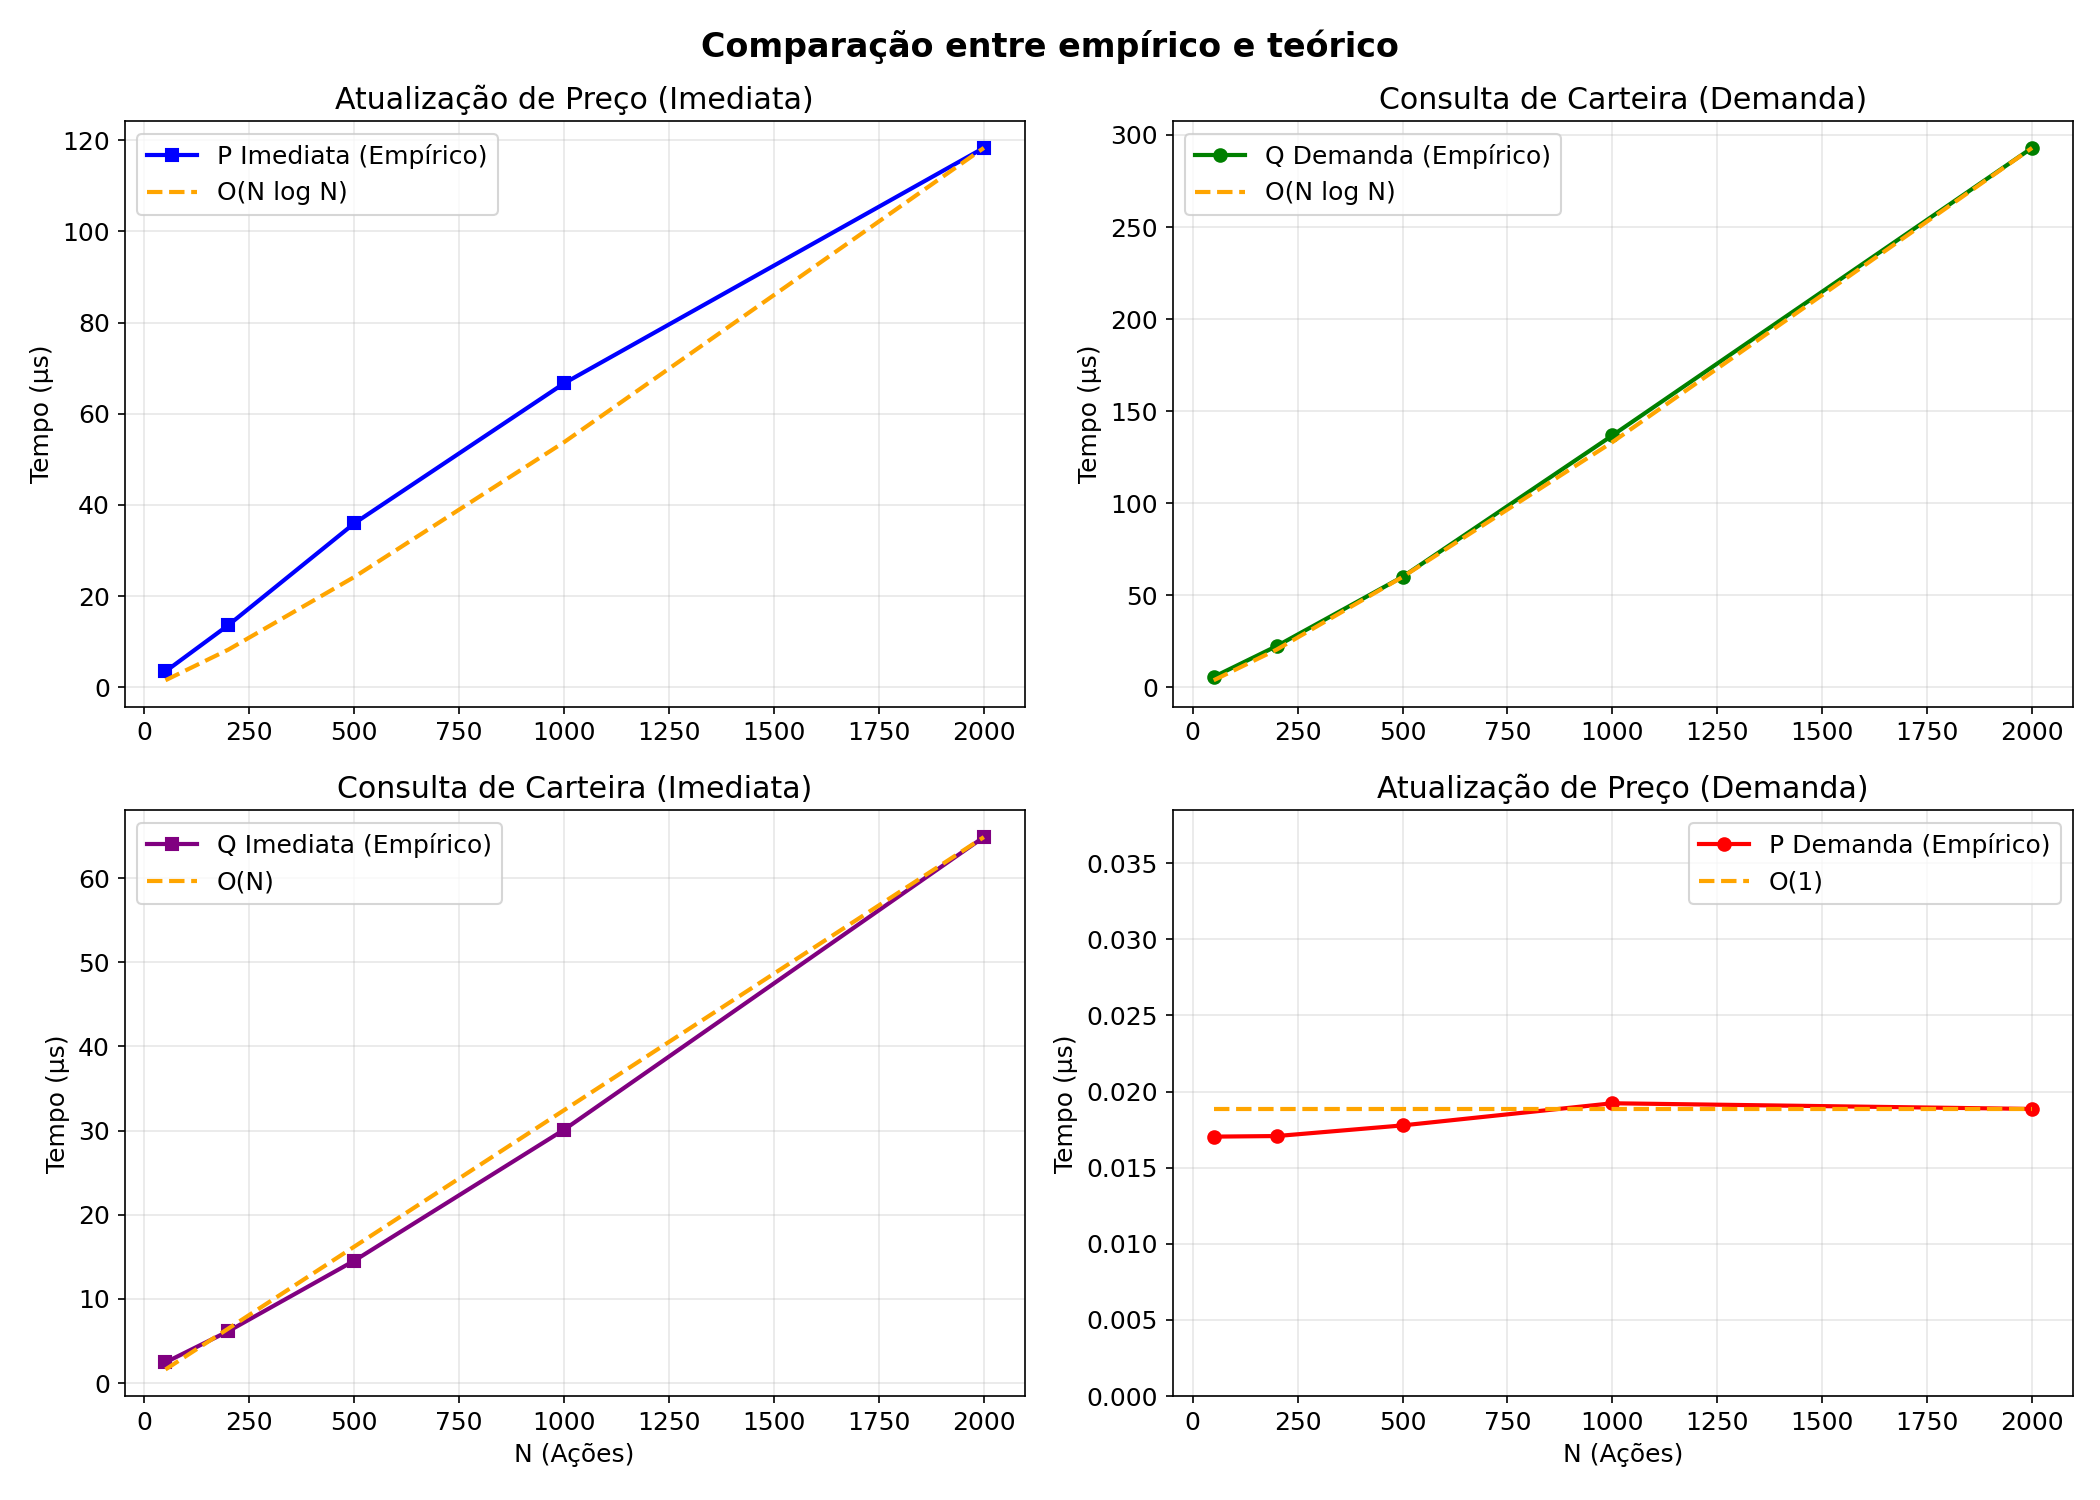
\includegraphics[width=0.7\linewidth]{grafico_assintotico.png}
    \caption{Comparação entre tempos empíricos e curvas de complexidade teórica.}
    \label{fig:assintotico}
\end{figure}

\subsection{Grupo A: Impacto da razão consultas/atualizações ($N_q/N_p$)}
Este grupo mantém $N=500$ e $w=10$ fixos e varia a proporção entre o número de consultas e atualizações de preço, de $N_q/N_p=0,01$ até $N_q/N_p=100$.

Como esperado, a estratégia sob demanda cresce com o número de consultas, enquanto a imediata decresce. Com $N_q/N_p=0,01$ (poucas consultas, muitas atualizações), a sob demanda completou em 7,0ms enquanto a imediata levou 655,4ms. Com $N_q/N_p=100$ (muitas consultas, poucas atualizações), a situação se inverte: a sob demanda levou 581,4ms contra 215,3ms da imediata.

O ponto de cruzamento ocorre entre $N_q/N_p=1$ e $N_q/N_p=10$. Com razão 1,0, a sob demanda leva 302,7ms e a imediata 435,7ms (sob demanda ainda vence). Com razão 10, a sob demanda sobe para 521,8ms e a imediata cai para 257,3ms, ou seja, imediata passa a ser mais eficiente.
\begin{table}[H]
\centering
\begin{tabular}{|c|c|c|}
\hline
\textbf{$N_q/N_p$} & \textbf{Sob demanda (ms)} & \textbf{Imediata (ms)} \\ \hline
0,01 & 7,0 & 655,4 \\ \hline
0,1  & 58,2 & 602,6 \\ \hline
1,0  & 302,7 & 435,7 \\ \hline
10   & 521,8 & 257,3 \\ \hline
100  & 581,4 & 215,3 \\ \hline
\end{tabular}
\label{tab:crossover}
\caption{Tempo total de execução por estratégia em função da razão $N_q/N_p$.}

\end{table}
\begin{figure}[H]
    \centering
    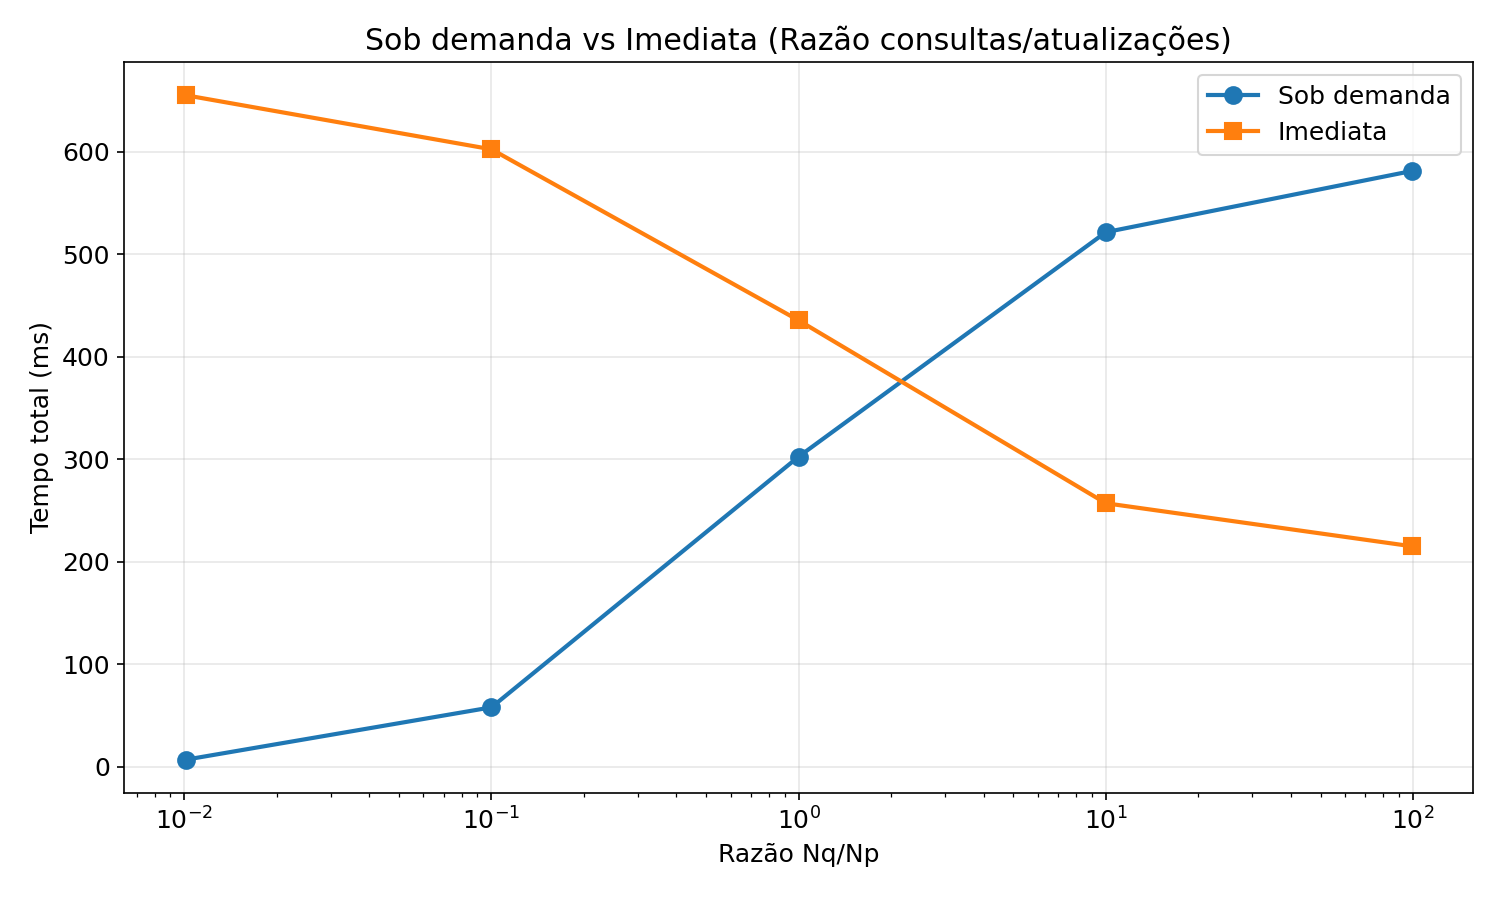
\includegraphics[width=0.7\linewidth]{grafico_crossover.png}
    \caption{Ponto de equilíbrio entre as estratégias Sob Demanda e Imediata.}
    \label{fig:crossover}
\end{figure}

\subsection{Grupo B: Impacto do número de ações ($N$)}
Este grupo mantém $w=10$ fixo com 5000 atualizações e 500 consultas, variando $N$ de 50 a 2000.

O tempo médio por consulta na sob demanda cresce de 5,6$\mu$s ($N=50$) para 293,0$\mu$s ($N=2000$), comportamento consistente com $\mathcal{O}(N \log N)$. O tempo médio por consulta na imediata cresce de 2,5$\mu$s para 64,9$\mu$s no mesmo intervalo, consistente com $\mathcal{O}(N)$.

O tempo médio por atualização na imediata cresce de 3,5$\mu$s ($N=50$) para 118,3$\mu$s ($N=2000$), também consistente com $\mathcal{O}(N \log N)$. Na sob demanda, o tempo por atualização permanece em torno de 0,017$\mu$s a 0,019$\mu$s independentemente de $N$, confirmando o comportamento $\mathcal{O}(1)$.

Para $N=2000$, a imediata leva 2991ms no total contra 147ms da sob demanda, uma diferença de 20x nesse cenário com poucas consultas relativas. Isso mostra que a imediata é desvantajosa quando $N$ é grande e as consultas são pouco frequentes.
\begin{table}[H]
\centering
\begin{tabular}{|c|c|c|c|c|}
\hline
\textbf{N} & \textbf{P demanda ($\mu$s)} & \textbf{P imediata ($\mu$s)} & \textbf{Q demanda ($\mu$s)} & \textbf{Q imediata ($\mu$s)} \\ \hline
50   & 0,017 & 3,5   & 5,6   & 2,5  \\ \hline
200  & 0,017 & 13,6  & 22,3  & 6,2  \\ \hline
500  & 0,018 & 36,0  & 59,9  & 14,5 \\ \hline
1000 & 0,019 & 66,7  & 136,8 & 30,1 \\ \hline
2000 & 0,019 & 118,3 & 293,0 & 64,9 \\ \hline
\end{tabular}
\caption{Tempo médio por operação em função de $N$.}
\label{tab:escala}
\end{table}
\begin{figure}[H]
    \centering
    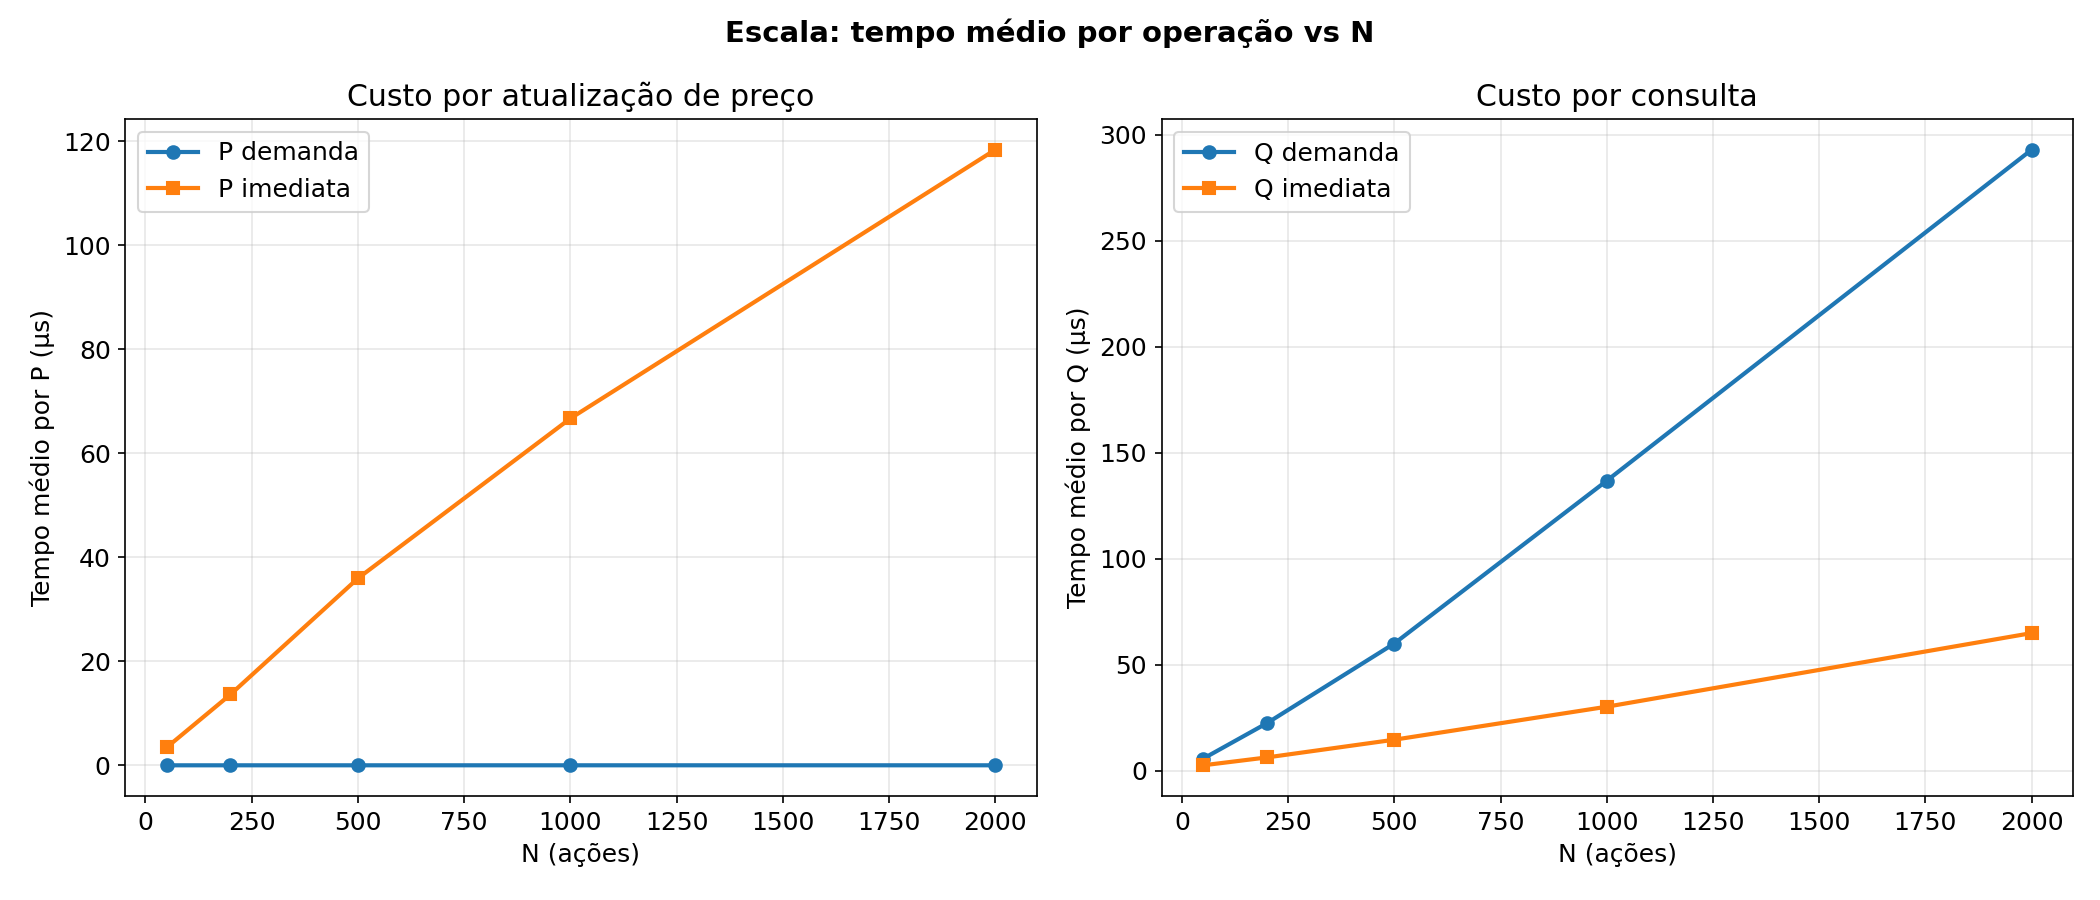
\includegraphics[width=0.7\linewidth]{grafico_escala.png}
    \caption{Impacto da variação do número de ações no tempo de execução.}
    \label{fig:escala}
\end{figure}

\subsection{Grupo C: Impacto do tamanho da janela ($w$)}
Este grupo mantém $N=500$ fixo com 5000 atualizações e 500 consultas, variando $w$ de 2 a 200.

A sob demanda é pouco afetada por $w$: o tempo total cresce de 23,6ms ($w=2$) para 177,9ms ($w=200$). Isso ocorre porque $\mathcal{O}(w)$ aparece no cálculo das métricas, mas é dominado pelo $\mathcal{O}(N \log N)$ do mergesort na consulta.

A imediata é muito mais sensível a $w$: o tempo total cresce de 186,4ms ($w=2$) para 3712,4ms ($w=200$), um aumento de quase 20x. Isso confirma que o termo $\mathcal{O}(w)$ pesa significativamente na estratégia imediata, pois o cálculo de métricas para todas as $N$ ações é executado a cada atualização de preço.
\begin{table}[H]
\centering
\begin{tabular}{|c|c|c|}
\hline
\textbf{$w$} & \textbf{Sob demanda (ms)} & \textbf{Imediata (ms)} \\ \hline
2   & 23,6  & 186,4  \\ \hline
10  & 30,3  & 369,7  \\ \hline
50  & 54,0  & 963,8  \\ \hline
200 & 177,9 & 3712,4 \\ \hline
\end{tabular}
\label{tab:janela}
\caption{Tempo total por estratégia em função de $w$.}
\end{table}
\begin{figure}[H]
    \centering
    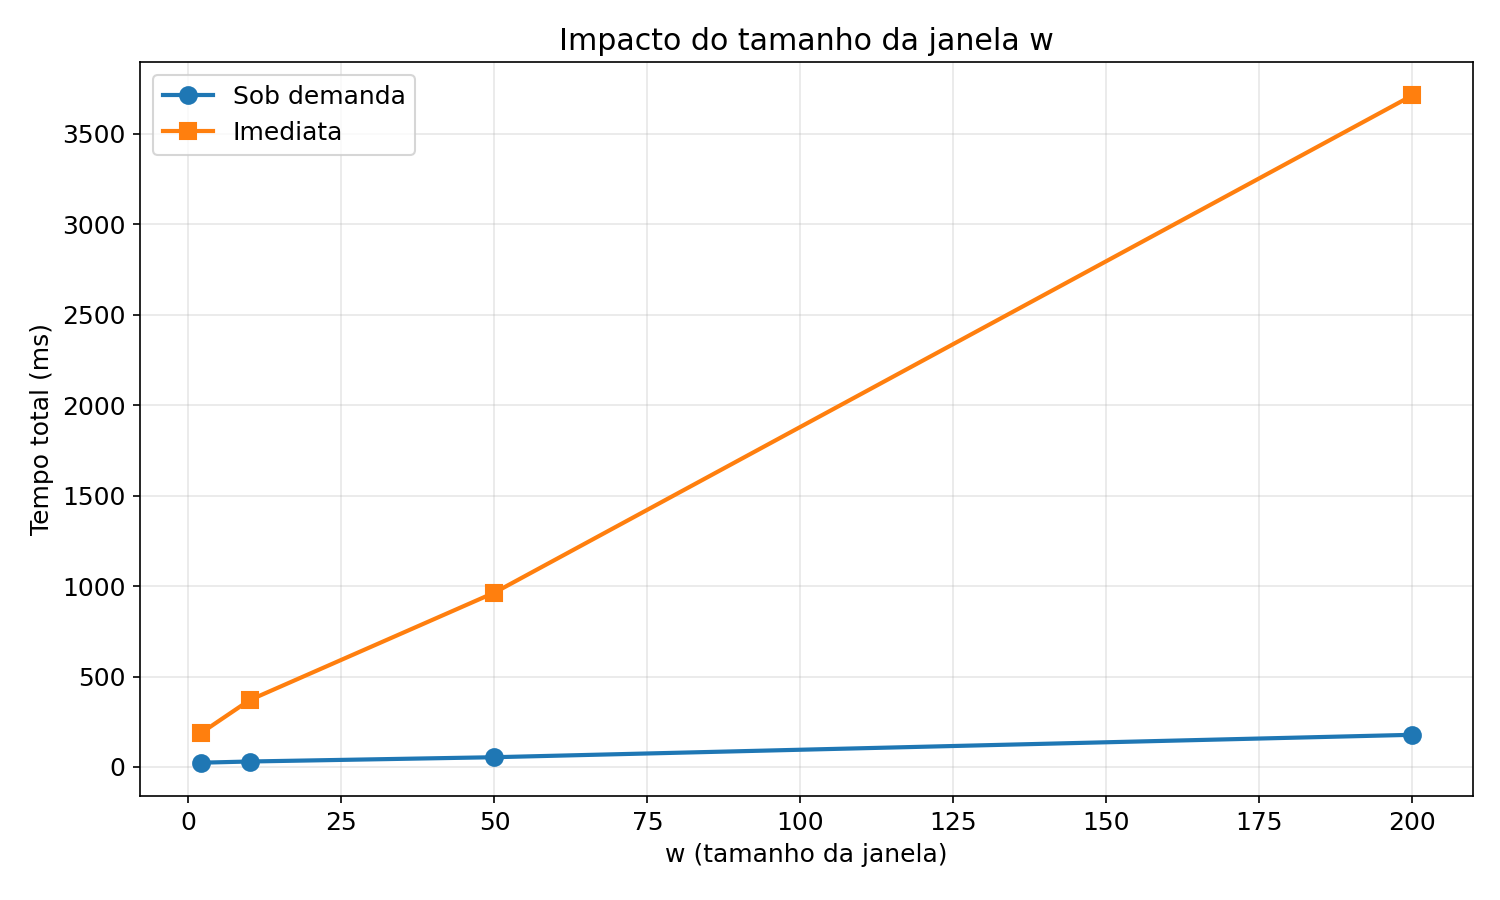
\includegraphics[width=0.7\linewidth]{grafico_janela.png}
    \caption{Impacto do tamanho da janela de cotações ($w$) no desempenho.}
    \label{fig:janela}
\end{figure}
\subsection{Conclusão da análise}
A estratégia sob demanda é superior quando atualizações são muito mais frequentes que consultas, ou quando $w$ é grande. A estratégia imediata compensa quando há muitas consultas por atualização. A inversão ocorre em torno de
 $N_q/N_p \approx 3$ a $5$ para $N=500$ e $w=10$. O parâmetro $w$ é o fator mais prejudicial para a imediata: janelas grandes tornam cada atualização muito cara, enquanto a sob demanda absorve esse custo de forma mais distribuída, pagando-o apenas nas consultas.
\section{Conclusões}
O sistema implementado atende aos requisitos do enunciado, com as duas estratégias de ranqueamento funcionando corretamente e produzindo os mesmos resultados. A parte mais trabalhosa foi acertar o buffer circular quando a janela ainda não estava cheia, já que as métricas davam resultados errados até a lógica de sentinela ser implementada. O array flat para as posições nos rankings também exigiu cuidado com a indexação, mas simplificou bastante o código de pontuação.

Na análise experimental, ficou claro que nenhuma das duas estratégias é melhor em todos os casos. A sob demanda funciona bem quando tem muita atualização e pouca consulta, e a imediata compensa quando as consultas são frequentes. O parâmetro $w$ acabou sendo o mais impactante pra estratégia imediata, já que janelas grandes tornam cada atualização de preço bem cara. Em suma, o principal aprendizado do projeto foi ver na prática como a escolha da estratégia computacional muda onde o sistema vai engasgar: não tem solução mágica, é sempre uma troca entre gastar tempo rodando cálculo na inserção ou na hora da busca.

\section{Bibliografia}
\bibitem{tp12026}
Anísio, Gisele, Wagner, Márcio (2026). \textit{Trabalho Prático 1: Análise Dinâmica de Carteiras de Ações}. Disponibilizado via Moodle. Departamento de Ciência da Computação. Universidade Federal de Minas Gerais. Belo Horizonte.
\bibitem{edslides2026}
Anísio, Gisele, Wagner, Márcio (2026). \textit{Slides da disciplina de Estrutura de Dados}. Disponibilizado via Moodle. Departamento de Ciência da Computação. Universidade Federal de Minas Gerais. Belo Horizonte.
\bibitem{abdulbari_channel}
BARI, Abdul. \textit{Abdul Bari - YouTube Channel}. Disponível em: <\url{https://www.youtube.com/@abdul_bari}>. Acesso em: 22 abr. 2026.

\end{document}
